\documentclass[10pt]{article}
\usepackage[top=1in, bottom=1in, right=1in, left=1in, nohead]{geometry}
\usepackage{amsmath}
\usepackage{graphicx}
\usepackage{subcaption}
\usepackage{float}
\usepackage{amsfonts}
\usepackage{listings}
\usepackage{pdfpages}
%%%%%%%%%%%%%%%%%%%%%%%%%%%%%%%%%%%%%%%%%%%
% MATLAB auto-generated code add-ons
\usepackage{color}
\sloppy
\definecolor{lightgray}{gray}{0.5}
\setlength{\parindent}{0pt}
%%%%%%%%%%%%%%%%%%%%%%%%%%%%%%%%%%%%%%%%%%%

\begin{document}

\title{MAE598: Design Optimization Homework 2}
\author{Tanner Bitz}
\maketitle

\includepdf[pages={1,2,3,4,5,6}]{Hw2_desopt_writeup}

\section*{Problem 2(b)}
\textbf{Implement the gradient descent and Newton’s algorithm
for solving the problem. Attach your codes in the report,
along with a short summary of your findings. The summary should
include: (1) The initial points tested; (2) corresponding solutions;
(3) A log-linear convergence plot. Based on your results, which
algorithm do you think is better? Why? Hint: A template can be
found here.}

\textbf{The Python Code for this section can be found at the end of this report.}



In my code, I start with the point $[x_2, x_3] = [-1, -1]$.  The objective function is strictly convex, so this optimization problem has a unique global minimum. This initial point, along with every other initial point I tested converges to the global minimum at $[x_1, x_2, x_3] = [-1.0714 -0.1429 0.7857]$. The value of the objective function at that point is 0.0714.  At this spot, the Gradient Descent algorithm took 96 iterations, and Newton's Method took 1 iteration.  I test at initial points as far as $[x_2, x_3] = [-10000, -10000]$ and it converged in about 150 iterations with Gradient Descent and 1 iteration with Newtons Method.  In the figures below, the paths going from [-1, -1] to the optimum are shown as well as a log-linear convergence plot. 

Determining which method is better depends on the contex of the problem.  If the objective function in not convex or the Hessian of the objective function is singular, then Newton's Method will not go to the optimum solution.  In these case, Gradient Descent should be used as it is proven to converge to a local minimum.  It should be noted that it will only be converge to a local minimum and not necessarily to a global minimum, but that is better than not converging at all.  The other consideration is the computational cost.  Newton's method has a higher computational cost per iteration as it has to compute the Hessian of the objective function as well as it's inverse, but it takes many many fewer iterations to converge to the global minimum as long as the objective function is convex.  For objective functions with many variables, the Hessian can grow large very quickly and thus Gradient Descent would likely be more computationally cheap despite required more iterations to converge. 

\begin{figure}[H]
  \centering
  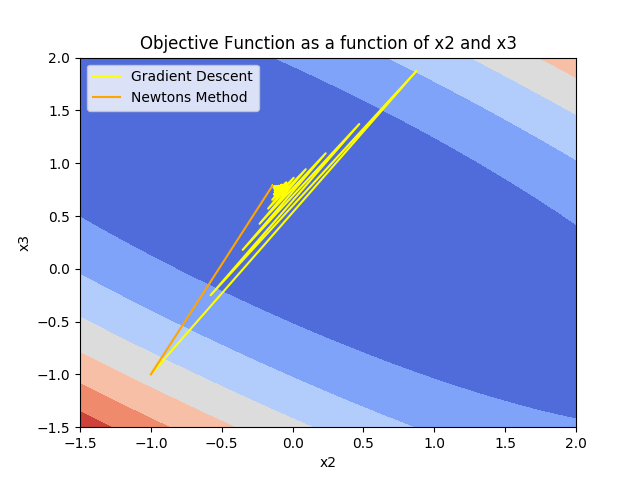
\includegraphics[width=.8\linewidth]{h2p2b_contourplot.png}
  \caption{Contour Plot with Paths to Optimum}
  \label{fig:sfig1}
\end{figure}
\begin{figure}[H]
  \centering
  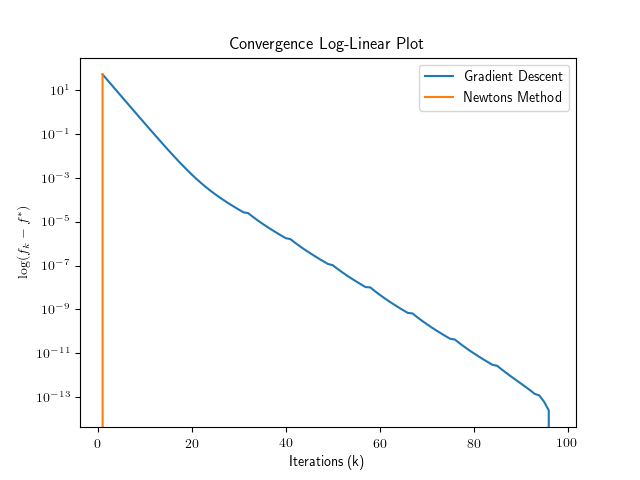
\includegraphics[width=.8\linewidth]{h2p2b_convergenceplot.png}
  \caption{Log-Linear Convergence Plot }
  \label{fig:sfig2}
\label{fig:fig}
\end{figure}



\includepdf[pages={7,8}]{Hw2_desopt_writeup}

\section*{Problem 4(b)}
\textbf{In what conditions will $f(g(x))$ be convex.}

In section 3.1.1 of Convex Optimization, Boyd, it is stated:

A function $f : R^n \to R $ is convex if dom f is a convex set and if for all x, y $\in$ dom f, and $\theta$ with $0 \leq \theta \leq 1$, we have 
$$
f(\theta x + (1-\theta) y) \leq \theta f(x) + (1-\theta) f(y)
$$ 

The part of interest in that statement is that the dom f must be convex.  From this, it is deteremined that for $f(g(x))$ to be convex, $g(x)$ must form a convex set. A function with any curvature is guaranteed to not form a convex set.  The trivial example of a parabola could be used to illustrate this point.  If two points on a the parabola are connected with a line, all of the points on the interior of that connecting line will not be in the set of points forming the parabola. Thus this wouldn't make a convex set.  Therefore, the only way that $f(g(x))$ would be convex is if $g(x)$ had no curvature which only occurs in some form/dimension of a hyperplane.  


\includepdf[pages={9}]{Hw2_desopt_writeup}



\section{Python Code}

\begin{lstlisting}[language=Python]
#!/usr/bin/python3
import numpy as np
import matplotlib.pyplot as plt
from mpl_toolkits.mplot3d import Axes3D
from matplotlib import cm, rc

#   Define the objective function f(x),
#   it's gradient g(x), and it's Hessian H(x)

#   Note: In homework problem x[0] == x2 and x[1] == x3
def f(x):
    return (2-2*x[0]-3*x[1])**2 + x[0]**2 + (x[1]-1)**2

def g(x):
    return np.array([-8, -14]) + np.array([[10, 12],[12, 20]]).dot(x)

def H(x):
    return np.array([[10, 12],[12, 20]]);

# Get the step direction based on method
def getStep(x):
    if prob['method'] == 'gradientDescent':
        s = -g(x)
    elif prob['method'] == 'newtonsMethod':
        s = -np.linalg.inv(H(x)).dot(g(x))
    return s


def getx1(x):
    # Get x1 value based on x2 and x3
    # x2 = x[0]
    # x3 = x[1]
    return 1 - 2*x[0] - 3*x[1]

def appendNewX(xarray, xnew):
    # Append new x vector to array of x at each iteration
    return np.concatenate((xarray, xnew))

def appendNewF(farray, fnew):
    # Add new value of f to solution array
    return np.append(farray, fnew)

def lineSearch(x0, prob, xiter, fiter):
    # x     - the initial x guess
    # prob  - the problem dict with settings
    # xiter - array of x values at iteration step
    # fiter - array of f values at iteration step
    iter = 0
    x = x0
    defaultAlpha = prob['a']
    while True:
        # If norm of gradient is greater than predefined
        # value, then break out of while loop.  Solution has converged.
        G = g(x)
        if np.linalg.norm(G, ord=2) < prob['eps']:
            break
        # If iteration count reaches maximum allowable iterations, then break
        if iter >= prob['itermax']:
            print("Solution did not converge in {} iterations using {}".format(
                    prob['itermax'],
                    prob['method']))
            break

        # Iterate
        s = getStep(x)
        fAlpha = f(x + prob['a']*s)
        phi = fiter[len(fiter)-1] + prob['a']*prob['t']*G.transpose().dot(s)
        while fAlpha > phi: # backtrack step if necessary
            prob['a'] = prob['b']*prob['a']
            fAlpha = f(x + prob['a']*s)
            phi = fiter[len(fiter)-1] + prob['a']*prob['t']*G.transpose().dot(s)
        # Set new position
        x = x + prob['a']*s

        # Save Necessary Iteration Data
        xiter = appendNewX(xiter, np.array([[getx1(x), x[0], x[1]]]))
        fiter = appendNewF(fiter, fAlpha)
        prob['a'] = defaultAlpha
        iter += 1

    return [iter, xiter, fiter]

############################################################
#                Set up Problem and Run                    #
############################################################

x0 = np.array([-1, -1]) # Initial Point

################## Gradient Descent ########################
xiter_g = np.array([[getx1(x0), x0[0], x0[1]]]) # value of x at each iteration
fiter_g = np.array([f(x0)]) # value of function at each iteration

prob = {
        'eps': 1e-6,
        'method': 'gradientDescent',
        'a': 1,
        't': 0.01,
        'b': 0.5,
        'itermax': 10000,
        }

[iterationsToFinish_g, xiter_g, fiter_g] = lineSearch(x0, prob, xiter_g, fiter_g)


print("The global minimum occurs at the point \n{}".format(xiter_g[len(xiter_g)-1]))
print("The minimum value of the objective function is {}".format(fiter_g[len(fiter_g)-1]))
print("The solution was found in {} iterations\n".format(iterationsToFinish_g))




###########              Newton's Method                   #############
xiter_n = np.array([[getx1(x0), x0[0], x0[1]]]) # value of x at each iteration
fiter_n = np.array([f(x0)]) # value of function at each iteration

prob = {
        'eps': 1e-6,
        'method': 'newtonsMethod',
        'a': 1,
        't': 0.01,
        'b': 0.5,
        'itermax': 10000,
        }

[iterationsToFinish_n, xiter_n, fiter_n] = lineSearch(x0, prob, xiter_n, fiter_n)

print("The global minimum occurs at the point \n{}".format(xiter_n[len(xiter_n)-1]))
print("The minimum value of the objective function is {}".format(fiter_n[len(fiter_n)-1]))
print("The solution was found in {} iterations.".format(iterationsToFinish_n))



# Contour Plot of Objective Function Minimization
fig = plt.figure()
ax = fig.add_subplot(111)
x = np.linspace(-1.5, 2.0, 100)
y = np.linspace(-1.5, 2.0, 100)
X, Y = np.meshgrid(x, y)
F = np.zeros(X.shape)
[ix, jx] = X.shape
for i in range(0, ix):
    for j in range(0, jx):
        F[i,j] = f(np.array([X[i,j], Y[i,j]]))

surf = ax.contourf(X, Y, F, cmap=cm.coolwarm)
plotgraddescentpath = ax.plot(xiter_g[:, 1], xiter_g[:, 2], color='yellow', label='Gradient Descent')
plotnewtonsmethodpath = ax.plot(xiter_n[:,1], xiter_n[:, 2], color='orange', label='Newtons Method')
plt.xlabel('x2')
plt.ylabel('x3')
plt.title('Objective Function as a function of x2 and x3')
ax.legend()

plt.show()


# Log linear convergence plot
fdist = fiter_g - fiter_g[len(fiter_g)-1]
x = np.arange(1, len(fdist)+1)
fdist_n = fiter_n - fiter_n[len(fiter_n)-1]
x_n = np.arange(1, len(fdist_n)+1)

fig2 = plt.figure()
plt.rc('text', usetex=True)
plt.semilogy(x, fdist, label='Gradient Descent')
plt.semilogy(x_n, fdist_n, label='Newtons Method')
plt.xlabel('Iterations (k)')
plt.ylabel(r'$\log (f_k-f^*)$')
plt.legend()
plt.title('Convergence Log-Linear Plot')
plt.show()




\end{lstlisting}


\end{document}